\subsubsection*{Dining Philosophers (DP)}

% \begin{figure}[tb]
% \centering
% \epsfig{file=eps/dining.eps,width=0.3\columnwidth}
% \caption{Three Dining Philosophers Problem.
% $A,B,C$ are philosophers while $x,y,z$ are forks.}
% \label{fig:dining}
% \end{figure}

% \RY{can delete the figure. Listing 9 can be joined horizontally rather
% than vertically as now}

Consider the well-known ``Dining Philosophers Problem''
\cite{Dijkstra2002:Hierarchical} - there are three
philosophers $A$, $B$ and $C$, sitting around a dining table,
with three forks $x$, $y$ and $z$ between them.
This classic concurrency problem
shows that deadlock happens with certain sequences of acquiring the forks,
e.g., $A$ acquires $x$, $B$ acquires $y$ and then
$C$ acquires $z$. 
The classic solution to this problem is using a synchronization mechanism 
such as a counting semaphore, imposing a partial order on acquiring the forks, 
or requiring one philosopher to be asymmetric.
However, such kind of solution requires additional constraints to the problem. 
%
In this example, the speculation framework offers an alternative
solution which is purely based on the definition of the problem.
We extend the problem to $N$ dining philosophers 
sitting around a table with $N$ forks.
For simplicity, each philosopher has a unique index ranging from $0$ to $N-1$. 
Listing \ref{lst:dpinit} shows the initialization of data stores 
for dining philosophers.
Listing \ref{lst:dp} shows the agent program for dining philosophers.
\texttt{my\_index()} returns the index of the current philosopher.

\begin{figure}[tb]
\begin{lstlisting}[label=lst:dpinit,caption=Dining Philosophers (initialization)]
for I = 0 to N-1
  |$\Out$|(fork,I)
|$\exit$|
\end{lstlisting}
\begin{lstlisting}[label=lst:dp,caption={Dining Philosophers. \texttt{\%} denotes the modulo operation. {\tt ;} separates multiple statements in one line. $\Out$ is non-blocking in the tuple space data model, so we don't need choices for putting back forks.}]
L = my_index(); R = (L+1) % N
(|$\In$|(fork,L); |$\In$|(fork,R)) |$\oplus$| (|$\In$|(fork,R); |$\In$|(fork,L))
|$\cm$|
|$\Out$|(fork,L); |$\Out$|(fork,R)
|$\exit$|
\end{lstlisting}
\shrink
\shrink
\end{figure}

By using such kind of speculation, it can be guaranteed that 
there is always one world where nobody deadlocks. 
For example, assume $N=3$, the combination of the choices from three philosophers 
theoretically creates eight worlds as in Figure \ref{fig:diningrun} 
(though in practice some of the worlds may never be there due to pruning).

\begin{figure}
\centering\small
\Tree[.$\oplus_A$
    [.$\oplus_{B_1}$
        [.$\oplus_{C_1}$
            {$A\compact:-x$ \\ $\quad-y$ \\ $B\compact:-y$ \\ $\quad-z$ \\ $C\compact:-z$ \\ $\quad-x$ \\ $(w_1)$}
            {\bk$A\compact:-x$ \\ \bk$\quad-y$ \\ \bk$B\compact:-y$ \\ \bk$\quad-z$ \\ \bk$C\compact:-x$ \\ \bk$\quad-z$ \\ $(w_2)$}
        ][.$\oplus_{C_2}$
            {$A\compact:-x$ \\ $\quad-y$ \\ $B\compact:-z$ \\ $\quad-y$ \\ $C\compact:-z$ \\ $\quad-x$ \\ $(w_3)$}
            {\bk$A\compact:-x$ \\ \bk$\quad-y$ \\ \bk$B\compact:-z$ \\ \bk$\quad-y$ \\ \bk$C\compact:-x$ \\ \bk$\quad-z$ \\ $(w_4)$}
        ]
    ][.$\oplus_{C_3}$
        [.$\oplus_{B_2}$
            {$A\compact:-y$ \\ $\quad-x$ \\ $B\compact:-y$ \\ $\quad-z$ \\ $C\compact:-z$ \\ $\quad-x$ \\ $(w_5)$}
            {\bk$A\compact:-y$ \\ \bk$\quad-x$ \\ \bk$B\compact:-z$ \\ \bk$\quad-y$ \\ \bk$C\compact:-z$ \\ \bk$\quad-x$ \\ $(w_6)$}
        ][.$\oplus_{B_3}$
            {$A\compact:-y$ \\ $\quad-x$ \\ $B\compact:-y$ \\ $\quad-z$ \\ $C\compact:-x$ \\ $\quad-z$ \\ $(w_7)$}
            {\bk$A\compact:-y$ \\ \bk$\quad-x$ \\ \bk$B\compact:-z$ \\ \bk$\quad-y$ \\ \bk$C\compact:-x$ \\ \bk$\quad-z$ \\ $(w_8)$}
        ]
    ]
]
\caption{Three Dining Philosophers Problem (tree of choices). Minus sign ($-$) denotes taking the fork. Deadlock only happens in $w_1$ and $w_8$.}
\label{fig:diningrun}
\shrink
\end{figure}

There are many practical algorithms and applications (e.g., 2-phase locking)
that are special cases or extensions of the Dining Philosopher Problem (DPP). 
So we generalize DPP as follows.
\begin{definition}[Generalized Dining Philosopher Problem]
Given a set of resources $R$ which are available at the beginning, 
$n$ agents each interested in a subset of resources 
$R_i\subseteq R (1\le i\le n)$, and each agent is a two-phase process:
  \begin{enumerate}
    \item In the \emph{acquisition phase} the agent consumes every resource $r\in R_i$ in any order;
    \item In the \emph{release phase} the agent puts back every resource $r\in R_i$ in any order.
  \end{enumerate}
  $R_i$'s may overlap so the scheduler may produce a schedule which can cause deadlock 
among the agents.
\end{definition}

\begin{theorem} Generalized Dining Philosopher Problems do not deadlock 
using speculative nondeterminism.
\end{theorem}
\begin{proof}[Proof sketch]
% first show there is always a solution
First, we construct a combination of choices which will never deadlock. 
Fix an ordering of the elements in $R$, for example $r_1,r_2,\dots,r_m$ where $m=|R|$. 
For any agent $i$, it consumes $R_i$ in this fixed order. 
Then there will be races instead of deadlocks because there will not be the 
case that agent $i$ consumes $r_x$ and waits for $r_y$, and agent $j$ consumes
$r_y$ and waits for $r_x$ ($x<y$ and $y<x$ cannot be true at the same time). 
% then show the solution will not be pruned
Then it can be shown this combination will not be pruned by commits in an 
eventually blocking world due to the commit semantics described in rule \ref{rule:cm}. 
\end{proof}
